\section{Specyfikacja zewnętrzna}

\subsection{Wykorzystanie algorytmu}

Program został przygotowany zgodnie z myślą wykorzystania podobną do algorytmu sortowania znajdującego się w standardowej bibliotece wzorców (\texttt{std::sort()}). Wykorzystanie algorytmu odbywa się w kilku krokach:

\begin{enumerate}
	\item Dołączenie pliku nagłówkowego do projektu poprzez zastosowanie komendy:
	
	\begin{lstlisting}
#include "K_means.h"
	\end{lstlisting}
	
	\item Utworzenie elementu klasy szablonowej o konkretnym typie:
	
	\begin{lstlisting}
K_means<Typ_Danych> k_means;
	\end{lstlisting}

	Gdzie <Typ\textunderscore Danych> oznacza dowolny, dostarczony przez użytkownika typ danych.
	
	\item Wykonanie algorytmu grupowania k-średnich
	\begin{lstlisting}	
result = k_means.Group(first, last, distanceMeasure, groupAverage, k, MaxIterations, StopCondition, PrintOutput);
	\end{lstlisting}
	
	Elementem zwróconym będzie wektor iteratorów wskazujących na pierwsze elementy grup posortowanych elementów.
	
	\item Opcjonalnym krokiem jest wywołanie wyświetlenia elementów kolekcji za pomocą funkcji DisplayCollection. Aby funkcja działała poprawnie, elementy w zakresie muszą implementować operator <<.
	\begin{lstlisting}	
DisplayCollection(Iterator first, Iterator last)
	\end{lstlisting}
\end{enumerate}

\subsection{Opis parametrów wywołania funkcji Group}\label{parameters}

\begin{description}
	\item[first] -- jest iteratorem swobodnego dostępu (używanym w takich strukturach jak na przykład vector czy deque ze standardowej biblioteki wzorców) wskazującym na pierwszy element z grupowanego zakresu.
	\item[last] -- jest iteratorem swobodnego dostępu (używanym w takich strukturach jak na przykład vector czy deque ze standardowej biblioteki wzorców) wskazującym na ostatni element z grupowanego zakresu.
	\item[distanceMeasure] -- obiekt funkcyjny opisujący metrykę pomiędzy elementami danego typu. Więcej informacji można znaleźć w podrozdziale \ref{metric}.
	\item[groupAverage] -- obiekt funkcyjny opisujący funkcję uśredniającą elementy danego typu. Więcej informacji można znaleźć w podrozdziale \ref{avg}.
	\item[k] -- określa maksymalną liczbę iteracji algorytmu. W przypadku, gdy parametr \texttt{StopCondition} ustawiony jest na \texttt{StableState}, wartość tego parametru jest nieistotna.
	\item[StopCondition] -- określa warunek stopu (\ref{stop}). Jest to argument typu wyliczeniowego i przyjmuje jedną z 3 wartości:
	\begin{itemize}
		\item MaxIterations -- warunkiem stopu jest wykonanie odpowiedniej liczby iteracji (podanej w parametrze \texttt{k}).
		\item StableState -- program wykonuje się tak długo, aż w kolejnych iteracjach nie nastąpi zmiana przynależności do skupienia żadnego pośród wszystkich grupowanych elementów.
		\item Both -- połączenie powyższych. Program wykonuje się identycznie jak w przypadku \texttt{StableState}, jednak może się zakończyć wcześniej jeżeli została wykonana określona liczba iteracji.
	\end{itemize}
	\item[PrintOutput] -- określa, czy informacje o współrzędnych centroidów i przynależności punktów do skupień mają być wypisywane na strumień wyjściowy. Uwaga: może znacznie zwiększyć czas wykonywania algorytmu.
\end{description}

Przykładowe wywołanie funkcji dla wektora o elementach typu całkowitego:

	\begin{lstlisting}	
result = k_means.Group(vec.begin(), vec.end(), Point2D_distance(), Point2D_average(), 4, 3, StableState, false);
	\end{lstlisting}

Gdzie \texttt{vec} jest wektorem ze standardowej biblioteki wzorców zawierającym wartości typu \texttt{int}, a \texttt{Point2D\textunderscore distance()} i \texttt{Point2D\textunderscore average()} są obiektami funkcyjnymi stworzonymi zgodnie z zasadami opisanymi w podrozdziałach \ref{metric} i \ref{avg}.

\subsection{Opis parametrów wywołania funkcji DisplayCollection}

\begin{description}
	\item[first] -- jest iteratorem swobodnego dostępu (używanym w takich strukturach jak na przykład vector czy deque ze standardowej biblioteki wzorców) wskazującym na pierwszy element z grupowanego zakresu.
	\item[last] -- jest iteratorem swobodnego dostępu (używanym w takich strukturach jak na przykład vector czy deque ze standardowej biblioteki wzorców) wskazującym na ostatni element z grupowanego zakresu.
\end{description}

Przykładowe wywołanie funkcji dla wektora o elementach typu całkowitego:

\begin{lstlisting}	
k_means.DisplayCollection(vec.begin(), vec.end());
\end{lstlisting}

Gdzie \texttt{vec} jest wektorem ze standardowej biblioteki wzorców zawierającym wartości typu \texttt{int}.

\subsection{Przykład scenariusza użycia}

Dla poniższego kodu:

\begin{lstlisting}	
	K_means<Point_2D> k_means;
	vector<Point_2D> vec = vector<Point_2D>();
	
	//Fill vec with data
	
	k_means.DisplayCollection(vec.begin(), vec.end());
	
	auto result = k_means.Group(vec.begin(), vec.end(), Point2D_distance(), Point2D_average(), 3, 2, StableState, true);
	
	k_means.DisplayCollection(vec.begin(), vec.end());
\end{lstlisting}

Wynik działania będzie następujący:

\begin{figure}[h]
	\centering
	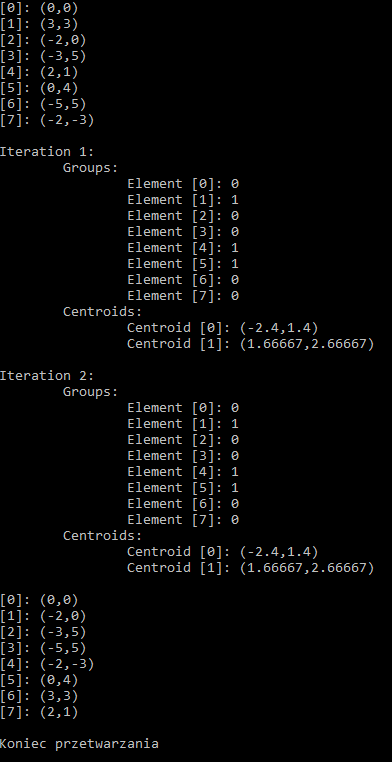
\includegraphics[width=0.35\textwidth]{./img/example.png}
	\caption{Przykładowe wywołanie algorytmu}
	\label{img:example}
\end{figure}